%%%%%%%%%%%%%%%%%%%%%%%%%%%%%%%%%%%%%%%%%%%%%%%%%%%%%%%%%%%%%%%%%%%%%
% LaTeX Template: Project Titlepage Modified (v 0.1) by rcx
%
% Original Source: http://www.howtotex.com
% Date: February 2014
%
% This is a title page template which be used for articles & reports.
%
% This is the modified version of the original Latex template from
% aforementioned website.
%
%%%%%%%%%%%%%%%%%%%%%%%%%%%%%%%%%%%%%%%%%%%%%%%%%%%%%%%%%%%%%%%%%%%%%%

\documentclass[12pt]{report}
\usepackage[a4paper]{geometry}
\usepackage[myheadings]{fullpage}
\usepackage{fancyhdr}
\usepackage{lastpage}
\usepackage{graphicx, wrapfig, subcaption, setspace, booktabs}
\graphicspath{ {img/} }
\usepackage[T1]{fontenc}
\usepackage[font=small, labelfont=bf]{caption}
\usepackage{fourier}
\usepackage[protrusion=true, expansion=true]{microtype}
\usepackage[english]{babel}
\usepackage{sectsty}
\usepackage{url, lipsum}
\usepackage{amsmath}
\usepackage{xfrac}
\usepackage{pgfgantt}
\usepackage{lscape}
\usepackage{url}
\usepackage{bm}
\setlength{\parindent}{0em}
\setlength{\parskip}{1.2em}

\newcommand{\HRule}[1]{\rule{\linewidth}{#1}}
\onehalfspacing

%-------------------------------------------------------------------------------
% HEADER & FOOTER
%-------------------------------------------------------------------------------
\pagestyle{fancy}
\fancyhf{}
\setlength\headheight{15pt}
\fancyhead[L]{Similar nodes in large graphs}
\fancyhead[R]{Vlad Velici}
\fancyfoot[R]{Page \thepage\ of \pageref{LastPage}}
%-------------------------------------------------------------------------------
% TITLE PAGE
%-------------------------------------------------------------------------------

%% USEFUL DEFINITIONS

\setcounter{secnumdepth}{2}
\setcounter{tocdepth}{3}

\renewcommand\thesection{\arabic{section}}
\renewcommand\thesubsection{\thesection.\arabic{subsection}}

\DeclareMathAlphabet{\mat}{OT1}{cmss}{bx}{12}

\begin{document}

\title{ \normalsize Electronics and Computer Science\\
Faculty of Physical Sciences and Engineering\\
University of Southampton
        \\ [2.0cm]
        Vlad Sebastian Velici \\
        \today
        \\ [1.0cm]
        {\LARGE \textbf{Similar nodes in large graphs}}
        \\ [1.0cm]
        Project Supervisor: Dr. Adam Prügel-Bennett \\
Second Examiner: Dr. Sasan Mahmoodi
	\\ [2.0cm]
	A project report submitted for the award of \\
MEng Computer Science with Artificial Intelligence
        \normalsize \vspace*{5\baselineskip}}

\date{}

\maketitle
\tableofcontents
\newpage

%-------------------------------------------------------------------------------
% ABSTRACT
%-------------------------------------------------------------------------------
\section*{Abstract}
%\addcontentsline{toc}{section}{Abstract}
Given a large graph, in the range of millions or billions of nodes, it is difficult
to efficiently find similar nodes. Examples of applications of finding similar
nodes in data represented as graphs are all around the web nowadays:
\textit{people you may know} and \textit{who to follow} suggestions on social
networks, or topics that may interest you on different websites.


This project will explore ways to obtain meaningful information of this nature
from large datasets represented as graphs.


The goals of this project are developing efficient ways to find similar nodes in
large graphs for different use cases and implementing an open-source software
library to provide everyone with this functionality.
\newpage
%-------------------------------------------------------------------------------
% INTRODUCTION
%-------------------------------------------------------------------------------
\section{Introduction}
%\addcontentsline{toc}{section}{Introduction}
%
Plenty of datasets are or can be represented as graphs where vertices represent
entities and edges represent relationships between entities. A problem of interest
is to find entities that are similarly connected. Example instances of this
problem are finding \textit{people you may know} in a social network, people with
common interests from research publications repositories or identifying possible
duplicates in a dataset.

It is possible to calculate cloud vectors that represent the neighbourhoods of
vertices in a graph only by looking at the structure of the graph. Then if a cloud
vector is close to another it means the vertices they represent belong to a similar
neighbourhood. Using the dot product of cloud vectors we can compute different
similarity measures between vertices. Cosine similarity and Euclidean distance
are studied in this report.

It is computationally too expensive to compute all the cloud vectors and then
the dot products or the Euclidean distances. This project investigates methods
for approximating the dot products, different similarity measures based on the
dot products, and the evaluation of these measures on real world datasets.


%
%-------------------------------------------------------------------------------
% CLOUD VECTORS AND SIMILARITY MEASURES
%-------------------------------------------------------------------------------
%
\section{Cloud vectors and similarity measures}

The cloud vector of a vertex represents the way this vertex is connected to the
rest of the graph. In other words, it represents an extended neighbourhood of the
node. It is created by a process similar to diffusion, as shown in
\emph{Figure~\ref{fig:ci_diffusion}}.

Given a graph $\mathcal{G}(\mathcal{V}, \mathcal{E})$ with adjacency matrix
$\mat{M}$. The number of nodes is $N = |v|$ and the number of edges is
$|\epsilon|$.

The cloud vectors represent the neighbourhoods of vertices of the graph
$\mathcal{G}$, thus looking at the number of walks of different lengths from a
vertex $i$ to all the other vertices in the graph is a promising start.

The adjacency matrix has the property that if it is raised to the $k^{th}$ power,
the $(i, j)$ element of it, $\mat{M}^k_{ij}$, is the number of walks of length
$k$ from vertex $i$ to vertex $j$. Therefore the $i^{th}$ column of $\mat{M}^k$
is a vector that represents the way vertex $i$ is connected to the rest of the
graph by walks of lenght $k$.

The could vectors should include the walks of all lengths with a preference
towards the shorter walks over the longer walks. Therefore the adjacency matrix
should be normalised such that all rows sum up to one. Let
%
\begin{equation}
\label{eq:initial-d}
\mat{D}_{ij} = \frac{\mat{M}_{ij}}{\sum_k^N \mat{M}_{ik}}
\end{equation}
be the normalised adjacency matrix. A matrix that includes walks of all lengths
as described above can be written as the sum
%
\begin{equation}
\label{eq:mu^t_d^t}
\sum_t^\infty \mu^t \mat{D}^t,
\end{equation}
%
where $\mu \in [0,1]$ is a penalising factor. For each vertex of the graph, $i
\in \mathcal{V}$, the cloud vector is the $i^{th}$ column of the matrix in
\emph{Equation~\ref{eq:mu^t_d^t}}, or mathematically
%
\begin{equation}
\label{eq:brute-ci}
\bm{c}_i = \sum_{t=0}^\infty \mu^t \mat{D}^t \bm{\delta}_i
\end{equation}
%
where $\bm{\delta}_i$ is the $i^{th}$ column of the $N \times N$ identity matrix.

\emph{Figure~\ref{fig:ci_diffusion}} shows the diffusion process of computing
$\bm{c}_i$ up to $k = 0, 1, 2, 3, 4, 5$. The coloured vertices are used in the
computation of $\bm{c}_i$ up to that $k$. The saturation of the colour of a vertex
$j$ represents the $j^{th}$ value of a normalised $\bm{c}_i$, such that red
represents the highest value in $\bm{c}_i$ and light gray represents values of 0.
In other words, the saturation of the colour of a vertex $j$ represents the strength
of the connection between vertex $i$ and vertex $j$. When $k=0$, only the first
vertex, $i$, counts. As $k$ gets larger, more and more vertices are considered
into the cloud vector $\bm{c}_i$, making it more accurate.

\begin{figure}[tpb]
  \centering
  \begin{subfigure}[b]{0.5\textwidth}
    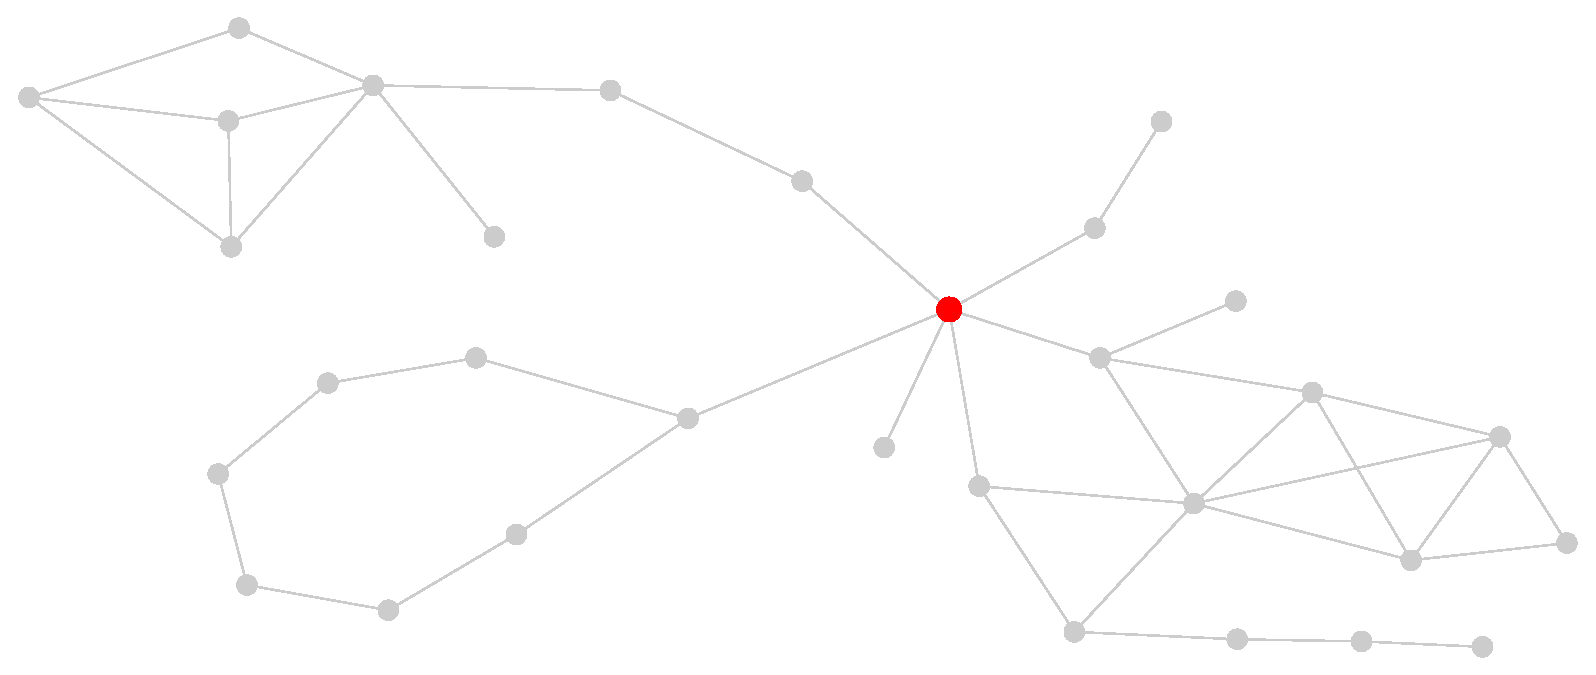
\includegraphics[width=\textwidth]{frame0}
		\caption{$k=0$}
    \label{fig:ci_diffusion_frame0}
  \end{subfigure}%
  ~
  \begin{subfigure}[b]{0.5\textwidth}
    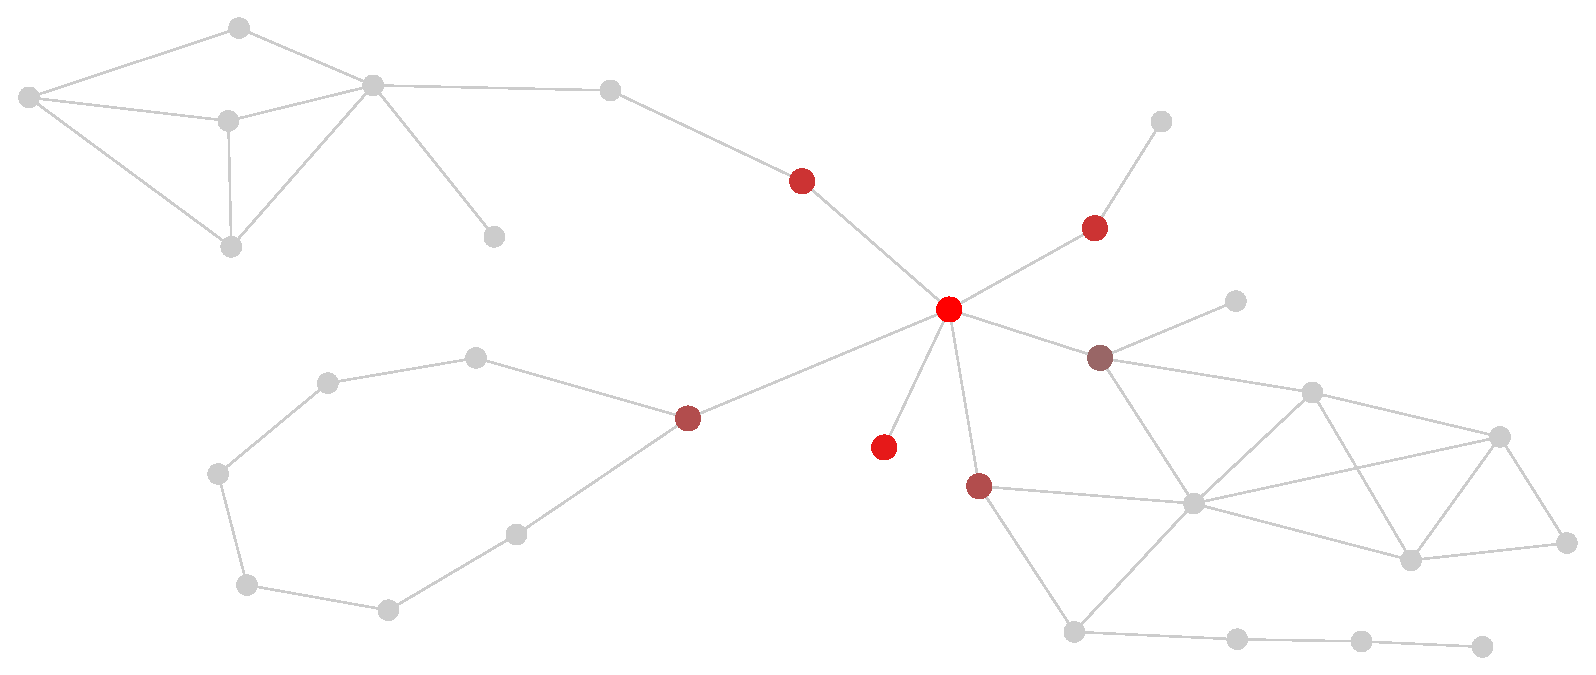
\includegraphics[width=\textwidth]{frame1}
    \caption{$k=1$}
  \end{subfigure}
  \begin{subfigure}[b]{0.5\textwidth}
    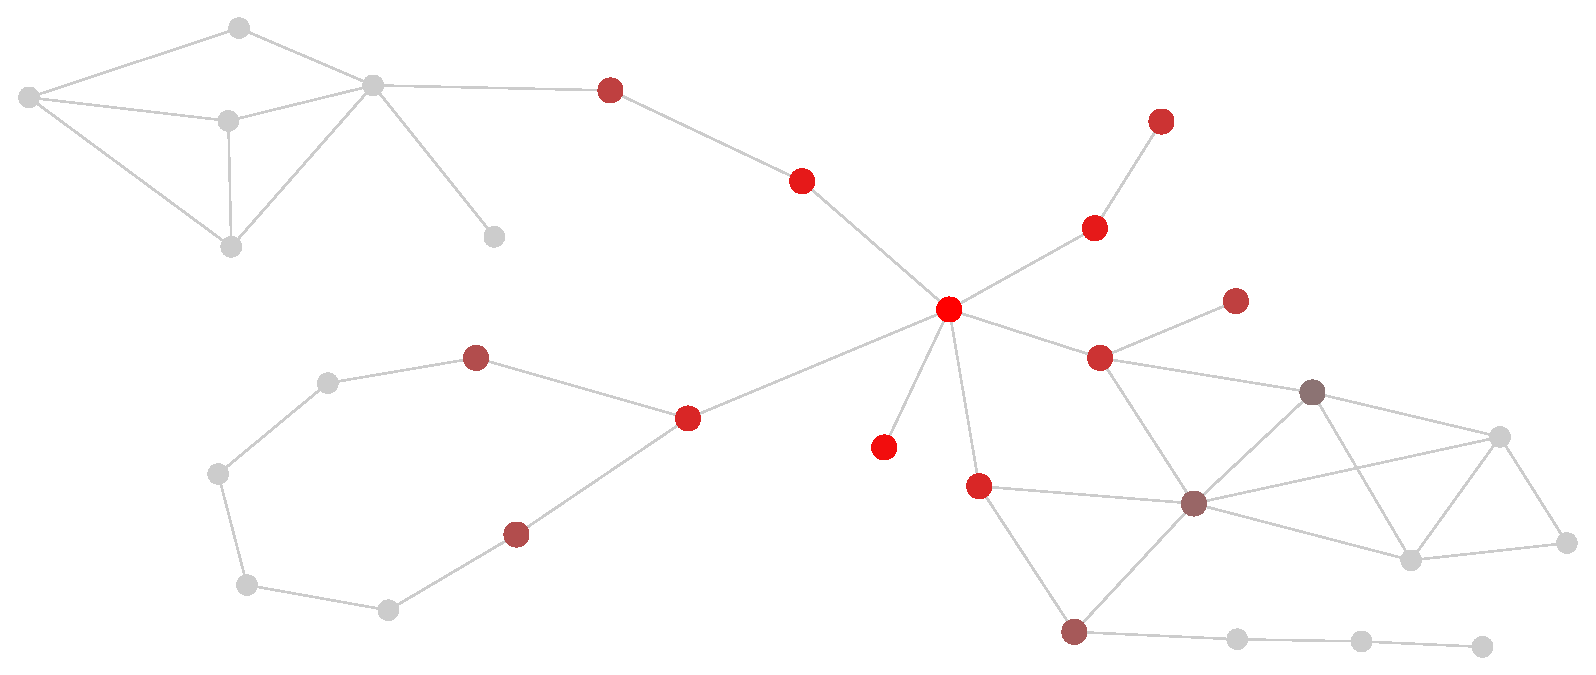
\includegraphics[width=\textwidth]{frame2}
		\caption{$k=2$}
  \end{subfigure}%
  ~
  \begin{subfigure}[b]{0.5\textwidth}
    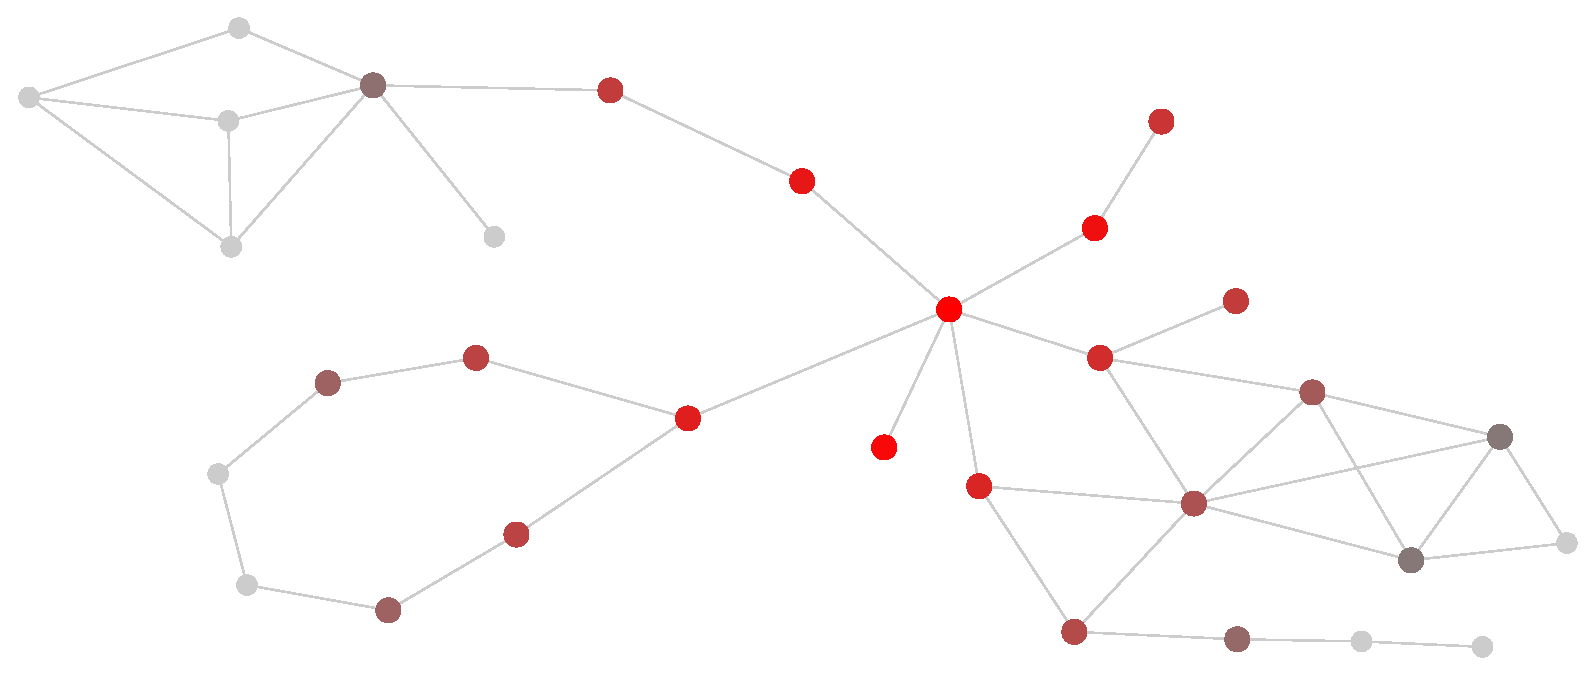
\includegraphics[width=\textwidth]{frame3}
    \caption{$k=3$}
  \end{subfigure}
  \begin{subfigure}[b]{0.5\textwidth}
    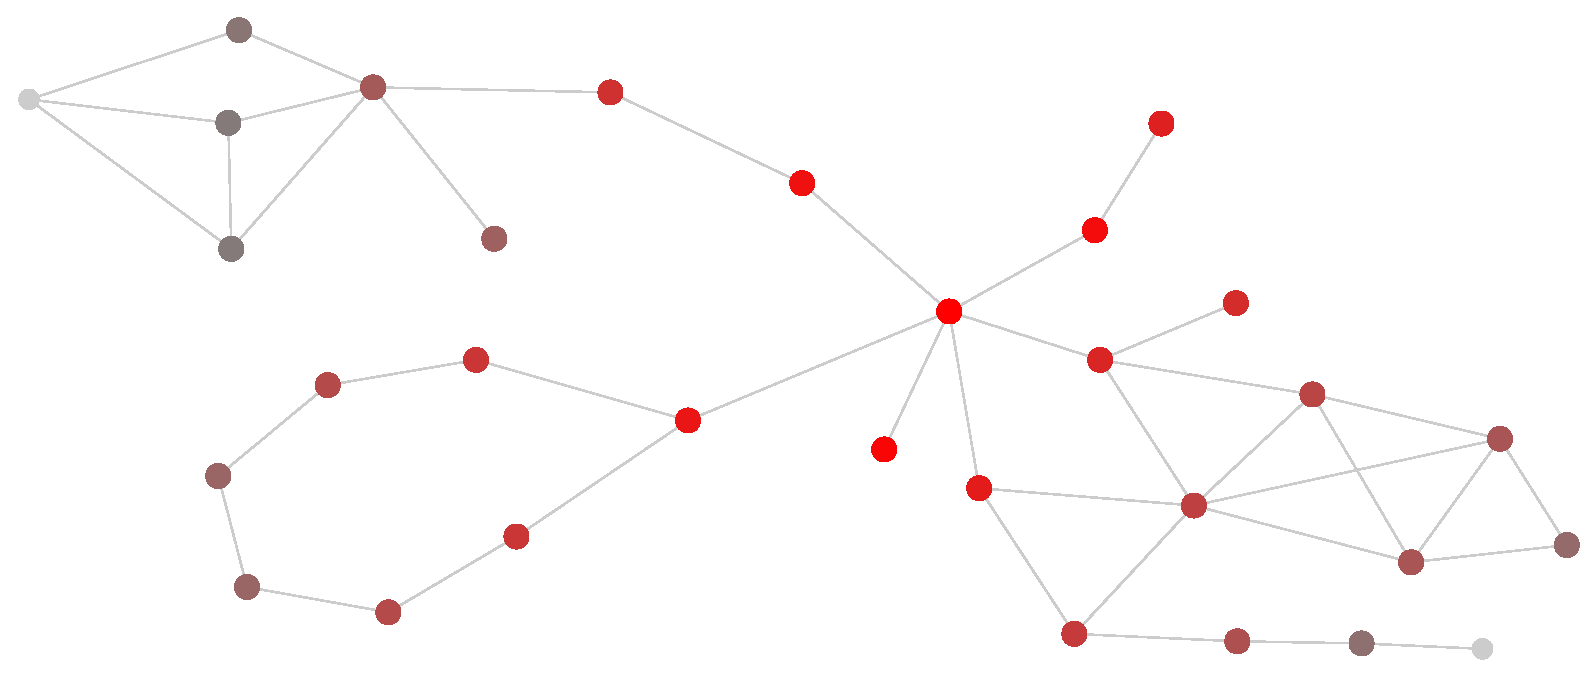
\includegraphics[width=\textwidth]{frame4}
		\caption{$k=4$}
  \end{subfigure}%
  ~
  \begin{subfigure}[b]{0.5\textwidth}
    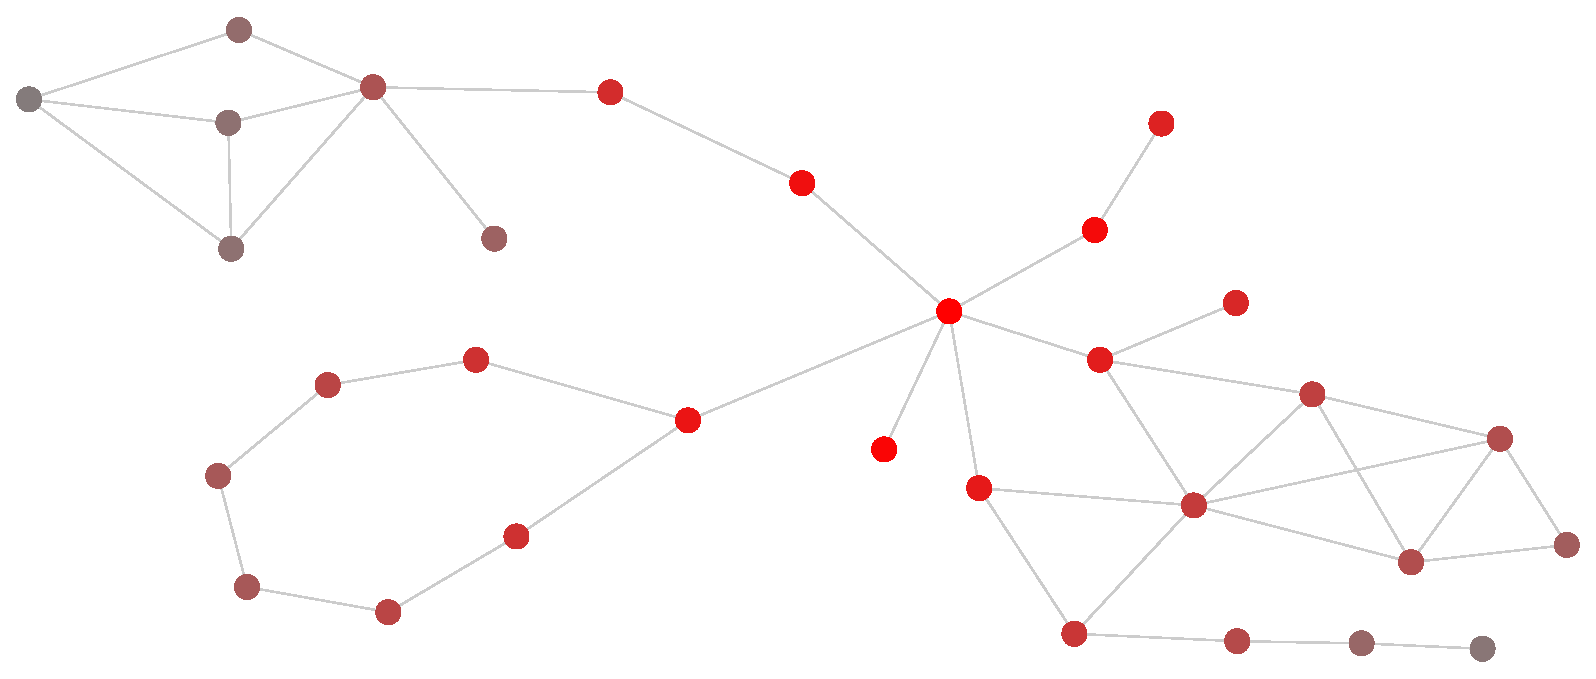
\includegraphics[width=\textwidth]{frame5}
    \caption{$k=5$}
  \end{subfigure}


  \caption{Computation of $\bm{c}_i = \sum_{t=0}^k 0.5^t \mat{D}^t \bm{\delta}_i$ up
  to different $k$. Vertex $i$ is the only red vertex in \textbf{(a)}. The
  saturation of the colour of a vertex, $j$, represents the connection strength
  between vertices $i$ and $j$ (red means strong connection and light gray no
  connection).}
  \label{fig:ci_diffusion}
\end{figure}

\subsection{Similarity between two vertices}

Two vertices of a graph are similar if they are in a similar neighbourhood. The
cloud vector of a vertex represents the neighbourhood of that vertex, therefore
the similarity between two vertices can be obtained by comparing their cloud
vectors.

One similarity measure is the Euclidean distance between cloud vectors. For
vertices $i$ and $j$ it is $\|\bm{c}_i - \bm{c}_j\|$. The smaller the distance
is, the more similar the vertices are. The minimum distance is $0$ and it is the
similarity between a vertex and itself.

Another similarity measure is the cosine similarity, which is the cosine of the
angle between the two vectors. It has values in the interval $[-1,1]$, with the
property that $\cos(0) = 1$ and $\cos(a) < \cos(b) \leq 1$, where $\pi \geq a > b
\geq 0$. A higher values means higher similarity, with $1$ being the maximum. The
cosine similarity ignores the magnitudes of the cloud vectors and only considers
the angle between them, therefore two cloud vectors that are not identical but
have the same direction (angle between them $0$) have the cosine similarity $1$.

%
%-------------------------------------------------------------------------------
% Naive implementation
%-------------------------------------------------------------------------------
%
\section{Naive approach}
%\addcontentsline{toc}{chapter}{Brute-force approach}
%
A naive implementation that does not scale to large graphs is to compute and
store all could vectors $\bm{c}_i, \forall i \in \mathcal{V}$. Observe that
\emph{Equation~\ref{eq:brute-ci}} is a geometric series and can be computed as
\begin{align}
  \label{eq:ci_inverse}
  \bm{c}_i = (\mat{I} - \mu \mat{D})^{-1} \bm{\delta}_i,
\end{align}
so every $\bm{c}_i$ vector is the $i^{th}$ column in the matrix $(\mat{I} -
\mu \mat{D})^{-1}$.

The naive approach was implemented and run on a small graph designed by hand and it gave
meaningful results (vertices connected to the graph in a similar way have a small
$\|\bm{c}_i - \bm{c}_j\|^2$) but it does not scale for large datasets.

Large graphs are expected to have sparse adjacency matrices, where the
number of edges is significantly lower then the number of vertices squared (
$|\mathcal{E}| \ll N^2$). The inverse $(\mat{I} - \mu \mat{D})^{-1}$ is
not sparse and it takes significantly more memory than the adjacency matrix. If
the graph is large enough, it can easily take more memory than the available RAM
on an average computer. Another problem is that computing the matrix inverse is
a computationally costly operation of complexity $O(N^3)$.

%
%-------------------------------------------------------------------------------
% Approximative approach
%-------------------------------------------------------------------------------
%
\section{Approximative approach}
%\addcontentsline{toc}{section}{Approximative approach}

%
%% Motivation for dot products only.
%
There are two similarity measures that should be computed, namely the Euclidean
distance between two cloud vectors and the cosine of the angle between them.

Geometrically, if vectors $\bm{c}_i$ and $\bm{c}_j$ start from the origin, then
$\bm{c}_i$, $\bm{c}_j$ and $\bm{c}_i-\bm{c}_j$ describe a triangle. Let $\theta$
be the angle between $\bm{c}_i$ and $\bm{c}_j$. From the Law of Cosines
%
\begin{equation}
  \label{eq:cosinelaw}
  \|\bm{c}_i-\bm{c}_j\|^2 = \|\bm{c}_i\|^2 + \|\bm{c}_j\|^2 - 2 \|\bm{c}_i\|
  \|\bm{c}_j\| \cos \ \theta.
\end{equation}
%
Take the dot product $\bm{c}^T_i\bm{c}_j = \| \bm{c}_i \| \| \bm{c}_j \| \cos \ \theta$.
The angle between $\bm{c}_i$ and itself is $0$ and $\cos \ 0=1$, thus
$\|\bm{c}_i\|^2 = \bm{c}^T_i\bm{c}_i$. Now \emph{Equation~\ref{eq:cosinelaw}} becomes
%
\begin{equation}
  \label{eq:norm-equation}
  \|\bm{c}_i-\bm{c}_j\|^2 = \bm{c}^T_i\bm{c}_i + \bm{c}^T_j\bm{c}_j - 2 \bm{c}^T_i\bm{c}_j,
\end{equation}
%
from which the Euclidean distance can be computed by taking the square root of the
result.

The cosine similarity can be computed using the same dot products
\begin{align}
  \cos \ \theta = \frac{\bm{c}^T_i\bm{c}_j}{\|\bm{c}_i\|\|\bm{c}_j\|} =
  \frac{\bm{c}^T_i\bm{c}_j}{\sqrt{\bm{c}^T_i\bm{c}_i} \ \sqrt{\bm{c}^T_j\bm{c}_j}}.
\end{align}

Therefore, it is sufficient to be able to compute all dot products $\bm{c}^T_i\bm{c}_j$
(for all $i, j \in v$) to compute the similarities between all vertices of the
graph. Computing and storing all $\bm{c}^T_i\bm{c}_j; i,j \in v$ takes too much
time and memory for a very large dataset, so we will make a trade-off between the
accuracy of the result and the computational complexity.


%
%% Approximative algorithm intro
%


An approximative algorithm to efficiently compute the dot products $\bm{c}^T_i\bm{c}_j$
will be described.

The algorithm is slightly different for directed and undirected graphs, because
undirected graphs have symmetric adjacency matrices. Symmetric matrices have the
advantage of having real eigenvalues, whereas non-symmetric matrices can have
both real and complex eigenvalues.

Both versions of the algorithm use the normalised adjacency matrix (from
\emph{Equation~\ref{eq:initial-d}}), which can be vectorised as
\begin{equation}
  \label{eq:d-vectorised}
  \mat{D} = \mat{W}\mat{M},
\end{equation}
where $\mat{W}$ is the diagonal matrix
\begin{equation}
  \label{eq:W}
  \mat{W}_{ii} = \frac{1}{\sum_{j=1}^N \mat{M}_{ij}}.
\end{equation}

%
%% Undirected graphs
%

\subsection{Undirected graphs}

In this subsection, assume that the graph $\mathcal{G}$ is undirected and, as a
consequence, the adjacency matrix $\mat{M}$ is a real symmetric matrix.

The normalised adjacency matrix $\mat{D}$ is not symmetric as it is the product
of a diagonal matrix ($\mat{W}$) and a symmetric matrix ($\mat{M}$). Knowing we
are interested in $\mat{D}^t$, define a new symmetric matrix
\begin{equation}
  \label{eq:a}
  \mat{A} = \mat{W}^{\sfrac{1}{2}}\mat{M}\mat{W}^{\sfrac{1}{2}}
\end{equation}
that can be used in
\begin{align}
  \label{eq:undirected-dt-waw}
  \mat{D}^t = (\mat{W}\mat{M})^t
      = \mat{W}^{\sfrac{1}{2}} \mat{A}^t \mat{W}^{\sfrac{-1}{2}}.
\end{align}

The matrices $\mat{W}^{\sfrac{1}{2}}$ and $\mat{W}^{\sfrac{-1}{2}}$ are easy to
compute because $\mat{W}$ is a diagonal matrix. Apply the operation only on the
diagonal elements and obtain $(\mat{W}^{\sfrac{1}{2}})_{ii} = (\mat{W}_{ii})^
{\sfrac{1}{2}}$ and $(\mat{W}^{\sfrac{-1}{2}})_{ii} = (\mat{W}_{ii})^
{\sfrac{-1}{2}}$.


%
%% Defining eigen*matrices.
%


Let $\lambda_i$ be the $i^{th}$ eigenvalue of $\mat{A}$ and $\bm{\vee^{(i)}}$ be
the $i^{th}$ eigenvector of $\mat{A}$ ($\forall i \in \{ 1, 2, ..., N \}$).
$\mat{V}$ is a matrix of all $N$ eigenvectors (such that $\bm{\vee^{(i)}}$ is
the $i^{th}$ column of $\bm{\vee}$), and $\bm{\Lambda}$ is a diagonal matrix
of all $N$ eigenvalues
%
\begin{align}
  \bm{\vee} &= \begin{bmatrix}
    \vert           & \vert           &       & \vert \\
    \bm{\vee^{(1)}} & \bm{\vee^{(2)}} & \dots & \bm{\vee^{(N)}} \\
    \vert           & \vert           &       & \vert \end{bmatrix}, &&
  \bm{\Lambda} = \begin{bmatrix}
    \lambda_1 & 0 		      & \dots  & 0 \\
    0 	 	    & \lambda_2   & \dots  & 0 \\
    \vdots 	  & \vdots	    & \ddots &   \\
    0	        & 0           &        & \lambda_N
  \end{bmatrix}.
\end{align}


%
%% Eigenvalue decomposition
%


The diagonalisation of the matrix $\mat{A}$ is $\mat{A} = \bm{\vee} \bm{\Lambda}
\bm{\vee}^{-1}$.
$\mat{A}$ is a real symmetric matrix thus its eigenvectors are orthogonal, which
makes $\bm{\vee}$ an orthogonal matrix, therefore $\bm{\vee}^{-1} = \bm{\vee}^{T}$
\cite{eigval_and_eigvec}. The diagonalisation of $\mat{A}$ is then
%
\begin{align}
  \mat{A} &= \bm{\vee} \bm{\Lambda} \bm{\vee}^{T} \\
  \Rightarrow \mat{A}^t &= \big(\bm{\vee} \bm{\Lambda} \bm{\vee}^{T}\big)^t
                  = \bm{\vee} \bm{\Lambda}^t \bm{\vee}^{T} \\
  \label{eq:a-at-t-sum}
                  &= \sum_{a=1}^{N} \lambda_a^t \bm{\vee^{(a)}} \bm{\vee^{(a)^T}}.
\end{align}


From \emph{Equation~\ref{eq:undirected-dt-waw}} and \emph{Equation~\ref{eq:a-at-t-sum}}
\begin{equation}
  \label{eq:d-at-t-with-a}
  \mat{D}^t = \mat{W}^{\sfrac{1}{2}} \sum_{a=1}^{N} \lambda_a^t \bm{\vee^{(a)}}
    \bm{\vee^{(a)^T}} \mat{W}^{\sfrac{-1}{2}}.
\end{equation}


%
%% Plugging into the Ci
%


Plug $\mat{D}^t$ from \emph{Equation~\ref{eq:d-at-t-with-a}} into
\emph{Equation~\ref{eq:brute-ci}}
\begin{equation}
  \bm{c}_i = \sum_{t=0}^\infty \mu^t \mat{W}^{\sfrac{1}{2}} \sum_{a=1}^{N}
    \lambda_a^t \bm{\vee^{(a)}} \bm{\vee^{(a)^T}} \mat{W}^{\sfrac{-1}{2}}
    \bm{\delta}_i,
\end{equation}
rearrange the equation and obtain
\begin{equation}
  \label{eq:ci-rearranged}
  \bm{c}_i = \mat{W}^{\sfrac{1}{2}} \sum_{a=1}^{N} \sum_{t=0}^\infty \mu^t
    \lambda_a^t \bm{\vee^{(a)}} \bm{\vee^{(a)^T}} \mat{W}^{\sfrac{-1}{2}}
    \bm{\delta}_i.
\end{equation}


%
%% Geometric series - to look into lambda mu < 1.
%


Note that $\sum_{t=0}^\infty \mu^t\lambda_a^t$ is a sum of a geometric series
with the first term $1$ and ratio $\mu \lambda_a$, therefore
\begin{equation}
  \label{eq:geometric-series}
  \sum_{t=0}^\infty \mu^t\lambda_a^t = \frac{1}{1 - \mu \lambda_a}.
\end{equation}


Observe $\bm{\vee^{(a)^T}} \mat{W}^{\sfrac{-1}{2}} \bm{\delta}_i$ is a scalar
\begin{equation}
  \label{eq:observe-scalar}
  \bm{\vee^{(a)^T}} \mat{W}^{\sfrac{-1}{2}} \bm{\delta}_i =
    \bm{\vee^{(a)}}_i \mat{W}^{\sfrac{-1}{2}}_{ii}.
\end{equation}


Substitute \emph{Equation~\ref{eq:observe-scalar}} and \emph{Equation~\ref{eq:geometric-series}}
back into \emph{Equation~\ref{eq:ci-rearranged}} and obtain
\begin{equation}
  \label{eq:ci-rearranged-geometric}
  \bm{c}_i = \mat{W}^{\sfrac{1}{2}} \sum_{a=1}^{N} \frac{1}{1 - \mu \lambda_a}
    \bm{\vee^{(a)}} \bm{\vee^{(a)}}_i \mat{W}^{\sfrac{-1}{2}}_{ii}.
\end{equation}


%
%% Approximation explained.
%


An approximation of the vectors $\bm{c}_i \ (\forall i \in \mathcal{V})$ can be
obtained by only using the $k$ leading eigenvectors and eigenvalues of $\mat{A}$
instead of all of them. It is expected that the $\mat{A}$ is large and sparse,
because in a typical dataset the number of relationships is significantly
smaller than the number of data points squared. In terms of the undirected graph
$\mathcal{G}(\mathcal{V}, \mathcal{E})$, it is expected that $\|\mathcal{E}\|
\ll \|\mathcal{V}\|^2$. The Lanczos Method is an efficient iterative algorithm
to compute the leading eigenvalues of large sparse real symmetric matrices
\cite{calvetti1994implicitly} and it is implemented in both Matlab and Python
(SciPy).

Compute the largest $k$ eigenvalues and eigenvectors using the Lanczos Method
and define $\bm{\hat{\vee}}$ to be the matrix of the $k$ leading eigenvectors
and $\bm{\hat{\Lambda}}$ to be the diagonal matrix of the leading $k$ leading
eigenvalues
\begin{align}
  \bm{\hat{\vee}} &= \begin{bmatrix}
    \vert           & \vert           &       & \vert \\
    \bm{\vee^{(1)}} & \bm{\vee^{(2)}} & \dots & \bm{\vee^{(k)}} \\
    \vert           & \vert           &       & \vert \end{bmatrix}, &&
  \bm{\hat{\Lambda}} = \begin{bmatrix}
    \lambda_1 & 0 		      & \dots  & 0 \\
    0 	 	    & \lambda_2   & \dots  & 0 \\
    \vdots 	  & \vdots	    & \ddots &   \\
    0	        & 0           &        & \lambda_k
  \end{bmatrix}.
\end{align}


Let $\bm{\hat{c}}_i$ be an approximation of $\bm{c}_i$
\begin{equation}
  \label{eq:c-hat}
  \bm{\hat{c}}_i = \mat{W}^{\sfrac{1}{2}} \sum_{a=1}^{k} \frac{1}{1 - \mu
    \lambda_a} \bm{\vee^{(a)}} \bm{\vee^{(a)}}_i \mat{W}^{\sfrac{-1}{2}}_{ii}.
\end{equation}


%
%% Define Z
%


To simplify the equation, let $\mat{Z}$ be a $N \times k$ matrix such that
\begin{align}
  \label{eq:z-ij}
  \mat{Z}_{ij} &= \frac{\bm{\vee^{(j)}}_i \mat{W}^{\sfrac{-1}{2}}_{ii}}
    {1-\mu \lambda_j},
\end{align}
and substitute in \emph{Equation~\ref{eq:c-hat}} to get
\begin{equation}
  \label{eq:ci-rearranged-z}
  \bm{\hat{c}}_i = W^{\sfrac{1}{2}} \sum_{a=1}^{N} Z_{ia} \bm{\vee^{(a)}}.
\end{equation}

The computation of $\mat{Z}$ (\emph{Equation~\ref{eq:z-ij}}) can be vectorised
using a new $k \times k$ diagonal matrix $\mat{R}$ as follows
\begin{align}
  \label{eq:z-vectorised}
  \mat{Z} = \mat{W}^{\sfrac{-1}{2}} \bm{\hat{\vee}} \mat{R}, &&
  \mat{R}_{ii} = \frac{1}{1 - \mu \lambda_i}.
\end{align}


%
%% Dot product undirected
%


The dot product between $\bm{\hat{c}}_i$ and $\mathbf{\hat{C}_j}$ becomes
\begin{align}
  \mathbf{\hat{C}_i^T} \mathbf{\hat{C}_j} &= \Big(  W^{\sfrac{1}{2}}
  \sum_{a=1}^{m} Z_{ia} \bm{\vee^{(a)}} \Big)^T \Big(  W^{\sfrac{1}{2}}
  \sum_{a'=1}^{m} Z_{ia'} \vee^{(a')} \Big)
  \\
  \Leftrightarrow \mathbf{\hat{C}_i^T} \mathbf{\hat{C}_j} &= \sum_{a=1}^{m} Z_{ia}  \bm{\vee^{(a)^T}} W \sum_{a'=1}^{m} Z_{ia'} \vee^{(a')}
  \\
\ Leftrightarrow \mathbf{\hat{C}_i^T} \mathbf{\hat{C}_j} &= \sum_{a=1}^m \sum_{a'=1}^m Z_{ia} Z_{ja'} \bm{\vee^{(a)^T}} W \vee^{(a')} \label{eq:dot-zvw}
\end{align}
%
%% Define Q
%
Define a new $m \times m$ matrix $Q$ such that:
%
\begin{equation}
\label{eq:q-ij}
Q_{ij} = \vee^{(i)^T} W \vee^{(j)}
\end{equation}
$\mathbf{Z_i}$ is the $i^{th}$ row of the matrix $\mat{Z}$. Substitute $Q$ into \emph{Equation~\ref{eq:dot-zvw}} and obtain:
\begin{align}
\mathbf{\hat{C}_i^T} \mathbf{\hat{C}_j} &= \sum_{a=1}^m \sum_{a'=1}^m Z_{ia} Z_{ja'} Q_{aa'} \label{eq:dot-zq-sum} \\
\Leftrightarrow \mathbf{\hat{C}_i^T} \mathbf{\hat{C}_j} &= \mathbf{Z_i^T} Q \mathbf{Z_j} \label{eq:dot-zq-vectorised}
\end{align}


\subsection{Directed graphs}

For directed graphs the Arnoldi Iteration \cite{lehoucq1996deflation} will be used
instead.

%
%% Storage and predictions
%
From \emph{Equation~\ref{eq:dot-zq-vectorised}} it is deduced that it is only
required to store the matrices $Q$ and $\mat{Z}$, which only takes $O(m^2 + Nm)$ memory,
instead of $O(N^2)$ to store all $\bm{\hat{c}}_i$ vectors.


To compute the similarity between two vertices, $i$ and $j$, use the norm formula
from \emph{Equation~\ref{eq:dot-zq-vectorised}} and obtain:
%
\begin{equation}
\|\mathbf{\hat{C}_i^T} - \mathbf{\hat{C}_j}\|^2 = \mathbf{Z_i^T} Q \mathbf{Z_i} + \mathbf{Z_j^T} Q \mathbf{Z_j} - 2 \mathbf{Z_i^T} Q \mathbf{Z_j}
\end{equation}
%
After computing the matrices $\mat{Z}$ and $Q$, the time complexity of computing the
similarity between two nodes is the same as multiplying three small matrices
(of sizes $1 \times m$, $m \times m$ and $m \times 1$).


%%%%%%%%%%%%%%%
%% Vectorisation
%%%%%%%%%%%%%%%
\subsection{Vectorisation}
%\addcontentsline{toc}{subsection}{Vectorisation}
It is usually more efficient to have vectorised implementations (to use matrix
operations in favour of iterative solutions) in programming languages like Matlab,
Octave or R. In this subsection is presented a way of computing the matrices $\mat{Z}$
and $Q$ using matrix operations. For this purpose, in this subsection, $\vee$ only
contains the leading $m$ eigenvectors (is of size $N \times m$), and $\Lambda$ only
contains the leading $m$ eigenvalues (is of size $m \times m$).


%
%% Z
%
To vectorise the computation of $\mat{Z}$ from \emph{Equation~\ref{eq:z-ij}}, define a
new diagonal matrix $R$:
%
\begin{equation}
R = \begin{bmatrix}
\frac{1}{1 - \mu \lambda_1} & 0  & \dots & 0 \\
0 & \frac{1}{1 - \mu \lambda_2}  & \dots & 0 \\
\vdots & \vdots & \ddots & \\
0 & 0 & \dots & \frac{1}{1 - \mu \lambda_m}
\end{bmatrix}
\end{equation}
And then define $\mat{Z}$ as:
\begin{equation}
Z = W^{\sfrac{-1}{2}} \vee R
\end{equation}
%
%% Q
%
A vectorised version of \emph{Equation~\ref{eq:q-ij}} (to compute $Q$) is:
\begin{equation}
Q = \vee^T W \vee
\end{equation}


%
%-------------------------------------------------------------------------------
% IMPLEMENTATION
%-------------------------------------------------------------------------------
\section{Implementation}
%\addcontentsline{toc}{section}{Implementation}
%
A choice had to be made on what tools and languages to use for the implementation
of this algorithm. It involves linear algebra so programming languages that support
such operations or have good libraries for this purpose were candidates. Matlab
was chosen for this task because it has very strong linear algebra features built-in,
it is easy and fast to try different experiments (can also be used interactively)
and programs are usually smaller in size (lines of code) than their variants in C++
or other languages. At a later stage when the algorithm is closer to its final
version, porting it to a language like Go or C++ will be considered.


Matlab has the function \textit{eigs(A,m)} to compute the leading $m$ eigenvectors
and eigenvalues \cite{matlab:eigs}. Internally, it uses the software package ARPACK which implements
implicitly restarted Arnoldi methods. \cite{lehoucq1998arpack}


Sparse matrices were used for the implementation of both the approximative and
the brute-force approaches. A sparse matrix in Matlab only stores the non-zero
values of a matrix, therefore a sparse matrix only uses memory for the positions
where it holds values\cite{gilbert1992sparse}. For instance, to store the adjacency matrix of a very
large graph $G(v,\epsilon)$, using a dense matrix would take $O(|v|^2)$ memory
whereas using a sparse matrix only takes $O(|\epsilon|)$ memory. Sparse matrices
are faster at linear algebra operations.


The approximative approach was implemented in Matlab as a couple of Matlab functions.
The function signatures along with descriptions is presented in \emph{Table~\ref{tbl:interface}}.
Some helper functions are not included in the table.
%
\begin{table}[!ht]\footnotesize
   \centering
   \begin{tabular}{ll}
   similarity(adj, mu, m) & Computes and returns the matrices Q and Z. \\
   sim2(q,z,i,j) & Computes the similarity between vertices i and j. \\
   simlist(q,z,i) & Computes the similarity between vertex i and all other vertices. \\
   top(q,z,i) & Uses simlist(q,z,i) and sorts the results. \\
   randomGraph(nodes, vertices, directed) & Generates a random connected graph.
   \end{tabular}
   \caption{Implementation interface. Parameters: q represents the matrix $Q$, z represents the matrix $\mat{Z}$, adj represents the adjacency matrix, and i and j represent vertex numbers.}
   \label{tbl:interface}
\end{table}


The brute-force algorithm was implemented as a separate set of Matlab functions
with a very similar interface.


%
%-------------------------------------------------------------------------------
% EVALUATION
%-------------------------------------------------------------------------------
%
\section{Evaluation}
%\addcontentsline{toc}{section}{Evaluation}
\subsection{Comparison of approximative and brute-force approaches}
%\addcontentsline{toc}{subsection}{Comparison of approximative and brute-force approaches}
%
A simple evaluation metric of how well the approximative approach retains the
most important information from the graph is to evaluate how different are the
top similar vertices for the brute-force approach and the approximative approach
with different number of eigenvalues and eigenvectors used.


For a dataset of $N$ vertices, let $B^m_{ij}$ be the position of vertex $j$ in
the top similar vertices of vertex $i$ for the brute-force approach with $m$
iterations. Similarly let $T^{m}_{ij}$ be the position of vertex $j$ in the top
similar vertices of vertex $i$ for the approximative approach with $m$ eigenvectors.
Define the difference between two such tops to be:
%
\begin{equation} d(B^m, T^{m'}) = \frac{1}{N^3} \sum_{i=1}^N \sum_{j=1}^N \operatorname{abs}(B^m_{ij} - T^{m'}_{ij}) \end{equation}
%
The equation is normalised by $N^3$ because the maximum value we can get lies in
the interval $(N^2, N^3)$.
%
\begin{figure}[tpb]
        \centering
        \begin{subfigure}[b]{0.6\textwidth}
	        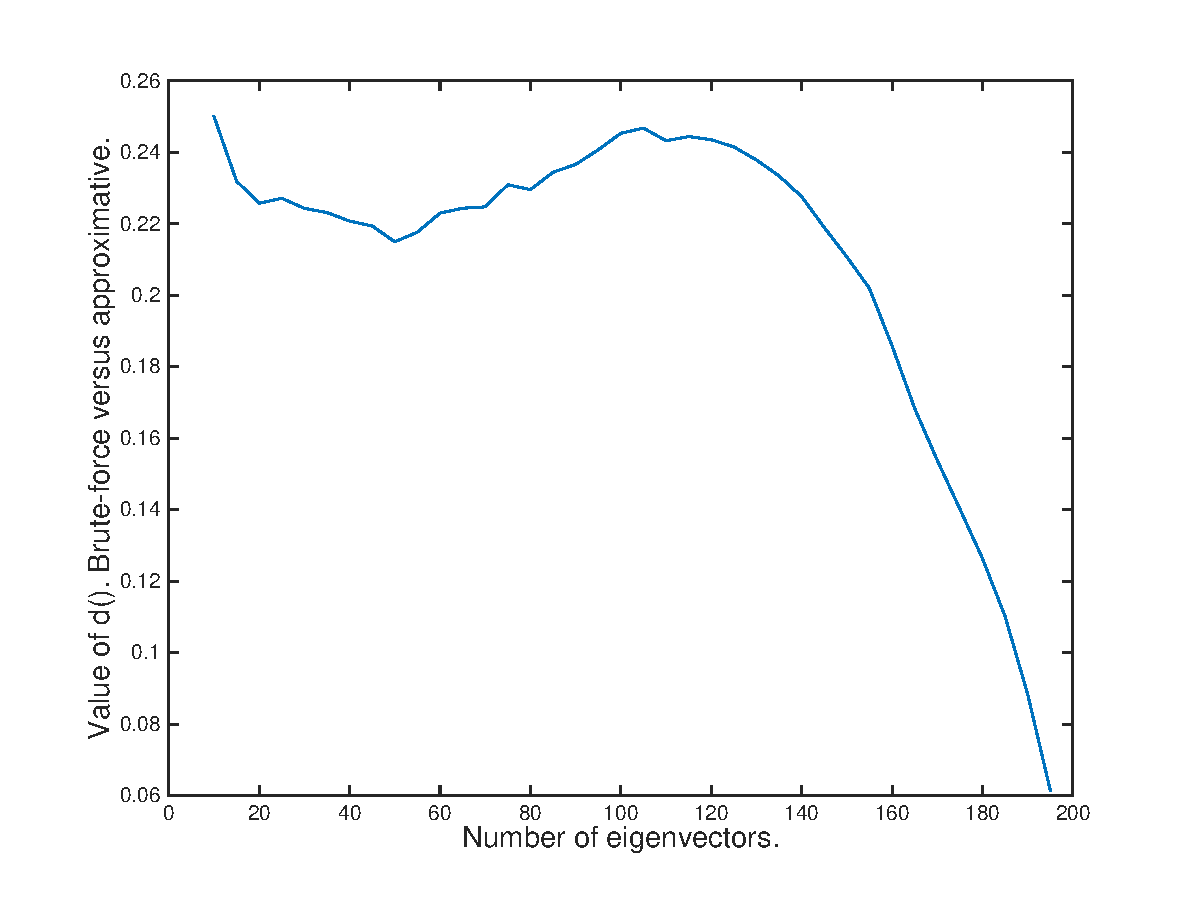
\includegraphics[width=\textwidth]{no-of-eigenvectors}
        		\caption{A plot of the differences on a range of eigenvalues.}
        \end{subfigure}%
        ~
        \begin{subfigure}[b]{0.4\textwidth}
           \centering
           \def\arraystretch{1.5}
           \begin{tabular}{|c|c|}
	   \hline
	   Parameters & Value of d() \\
	   \hline
	   $d(B^{20}, T^{10})$ & 0.2501 \\
	   \hline
	   $d(B^{20}, T^{20})$ & 0.2257   \\
	   \hline
   	   $d(B^{20}, T^{30})$ & 0.2243   \\
	   \hline
	   $d(B^{20}, T^{40})$ & 0.2208   \\
	   \hline
	   $d(B^{20}, T^{50})$ & 0.2150 \\
	   \hline
	   $d(B^{20}, T^{100})$ & 0.2453\\
	   \hline
	    $d(B^{20}$, $T^{199})$ & 0.0325 \\
	    \hline
	   \end{tabular}
	   \caption{Table of some of the values.}
	   \label{tbl:comparisons}
        \end{subfigure}%
        \caption{Difference of results between brute-force and approximative approaches.}
	\label{fig:no-of-eigenvectors}
\end{figure}
%


The value of $d()$ was evaluated on a randomly generated connected graph with $200$
vertices and $350$ edges, between the brute-force approach with $m=20$ iterations
and the approximative approach with $m' = 10$ to $199$ eigenvectors. The choice
of the penalising factor $\mu=0.5$ was used for all the runs. The results can be
observed in \emph{Figure~\ref{fig:no-of-eigenvectors}}. We can observe that if
we use the majority of eigenvalues, the value of $d()$ is very small. It is
computationally infeasible to do that on a large dataset thus we will aim for a
number of eigenvectors $m'$ in the range of $20$ to $40$, where the difference
seems to be at a local minimum (for this graph). The local minimum differs from
dataset to dataset depending mainly on the size of the dataset. For completeness,
the experiment was run on a randomly generated connected graph with $500$ vertices
and $700$ edges. The first local minimum of $d()$ was at around 100 eigenvectors
with a value of approx. $0.2$. At $40$ and $20$ eigenvectors, the values of $d()$
obtained are $0.2297$ and $0.2557$, respectively.


%
% -----
% Evaluation of the algorithm itself
% -----
%
Although the evaluation metric described above might be useful to compare the two
approaches directly, it does not tell anything about how well the algorithm achieves
its goal of finding similar entities in a real dataset. We will now examine ways to
evaluate the performance of the algorithm on real problems.


%
\subsection{Visualisation}
%\addcontentsline{toc}{subsection}{Visualisation}
%
A subjective method of evaluation on real data is attempting to visualise the
algorithm output on real data and deduce whether it gives sensitive results.
This method has the disadvantage of being subjective and it cannot scale to very
large graphs, but it might give a broad idea of what the results are and help
fine-tune the algorithm on specific problems.


%
\subsection{Discussion of further evaluation}
%\addcontentsline{toc}{subsection}{Discussion of further evaluation}
%
None of the evaluation methods described above give an objective, efficient and
automatic evaluation metric. In this subsection we discuss a few possible evaluation
methods of the algorithm.


To objectively evaluate how well the outputs of the algorithm reflect the reality
of the dataset it is being used on, we need to carefully define the goals of the
algorithm in respect of the dataset. We want labelled datasets where the natural
\textit{similarities} between entities is known and depends exclusively on the
graph structure. We do not want to evaluate how well the weights of different
relationship types are defined, thus the evaluation dataset must have only one
relationship type.


Given some datasets that fit the above requirements, we can run our algorithm and
compare the results with the reference (natural) similarities. In reality, datasets
have many features and natural \textit{similarities} between entities depend on many
features, thus this type of evaluation is not practical.


For specific tasks we can evaluate the performance of our algorithm by adding or
removing some edges from the graph. For instance, if we want to find duplicates
we can create a dummy vertex by duplicating an existing one and randomly removing
some of its edges. We then evaluate whether the dummy vertex is very similar to
the original vertex.


Implementing the evaluation method described above is included in the future plans
of this project, along with investigating more methods of evaluation.


%
%-------------------------------------------------------------------------------
% LIMITATIONS
%-------------------------------------------------------------------------------
%
\section{Limitations of current implementation}
%\addcontentsline{toc}{section}{Limitations of the current implementation}
%
The current implementation of this algorithm has various limitations which are
discussed along with possible improvements.


Directed graphs are not currently supported. In practice, datasets have meaningful
unidirectional relationships (e.g. in a social network person A follows person B,
but B does not follow A), and often datasets are represented as directed graphs
rather than undirected graphs. The algorithm can be adapted to support both directed
and undirected graphs but it will have the disadvantage of requiring to compute
$V^{-1}$ (for undirected graphs, $V^{-1} = V^T$).


In the real world datasets might have different types of relationships between
entities. Some relationship types might be more relevant than others in finding
a specific result. For instance, in a social network two people being friends
might be more relevant for recommending new friends than two people following the
same topic. The current implementation of the algorithm can compute similarities
if it is given a weighted (symmetric) adjacency matrix but it does not have a
way to automatically obtain (learn) these weights from the dataset.


What if the dataset is too large to fit into main memory? The algorithm is
currently designed to run only on one machine, but finding ways to distribute it
over multiple machines will help run it on even larger datasets.

%
%-------------------------------------------------------------------------------
% FUTURE PLANS
%-------------------------------------------------------------------------------
%
\section{Future plans}
%\addcontentsline{toc}{section}{Future plans}
%
The highest priority improvements are: develop a good evaluation method, add support
for directed graphs, and use different edge weights for different types of relationships.
A detailed plan can be observed in the Gantt Chart in \emph{Figure~\ref{fig:gan}}.


An evaluation method is not trivial to design and build for this algorithm, but
it is crucial to the validation, further development and fine-tuning of the algorithm.
Researching an evaluation model has the highest priority in the list of tasks.


Plenty of datasets on which this algorithm can be applied describe directed graphs
with multiple types of relationships. The relevant tasks are the next tasks in
the Gantt Chart.


A demo on one or more datasets will be built. The first step into getting feedback
and evaluating how the algorithm performs on real data is to build an interface
where users can interact with the results.


A small research on how to make the algorithm run on multiple machines will be
done. Also, if the time allows, the code will be ported to a language like Go or
C++ and released as an open-source project.
\begin{landscape}
\begin{figure}[ft]
\begin{center}
\begin{ganttchart}[vgrid=true, hgrid=true, y unit chart=1.5em, y unit title=1.4em, title height=1]{1}{32}
\gantttitle{Semester 1}{17} \gantttitle{Semester 2}{15} \\
\gantttitlelist{1,...,32}{1} \\
\ganttbar{Agreed project \& brief}{1}{2} \\
\ganttbar{Implemented brute-force}{3}{3} \\
\ganttbar{Understanding math.}{4}{9} \\
\ganttbar{Implementing approx.}{8}{10} \\
\ganttbar{Evaluation ideas}{10}{11} \\
\ganttbar{Write progress report}{11}{11} \\
\ganttmilestone{Progress report}{11} \\
\ganttbar{Research evaluation}{12}{19} \\
\ganttbar{Directed graphs support}{18}{21} \\
\ganttbar{Learn weights algorithm}{21}{25} \\
\ganttbar{Real datasets demo}{26}{28} \\
\ganttbar{Write final report}{28}{30} \\
\ganttmilestone{Final report}{30} \\
\ganttbar{Prepare Viva}{31}{32} \\
\ganttmilestone{Viva}{32}
\end{ganttchart}
\end{center}
\caption{Gantt Chart of done and planned tasks over weeks.}
\label{fig:gan}
\end{figure}
\end{landscape}

\newpage
\addcontentsline{toc}{section}{Bibliography}
\bibliography{ref.bib}{}
\bibliographystyle{plain}
\end{document}
